\documentclass[
  fontsize=10pt,
  %chapterprefix=true,
  numbers=noenddot,
  %draft,
]{../kaobook}

% Load common packages and commands
\usepackage{../style}
\usepackage{../packages}
\usepackage{../commands}

% Load packages for testing
\usepackage{blindtext}
%\usepackage{showframe}
%\usepackage{showlabels}

% Add bibfile
\addbibresource{main.bib}

% Set path for images
\graphicspath{{images/}{../images/}}

% Index
%\makeindex[columns=3, title=Alphabetical Index, intoc]

% Glossary
\makeglossaries

\begin{document}

% General structure of a book:
% 	\frontmatter
% 	Cover
% 	Half-title (r)
% 	Empty (v)
% 	Title (r)
%	Information (copyright, ISBN, etc.) (v)
%	Dedication (r)
%	Notation and other conventions used (v)
%	Table of contents (r)
%	List of figures (r)
%	Preface (r)
%
%	\mainmatter
%	Chapters (1, 2, ..., n)
%
%	\appendix
%	Appendices (A, B, ..., Z)
%
%	\backmatter
%	Bibliography (r)
%	Glossary (r)
%	Index (r)
%	Empty
%
%	Cover

\title{Title of the Book}
\author{Author Name}
\publishers{}
\date{}

\frontmatter

% Front cover
%\includepdf{pages/cover-front.pdf}

% Half-title

\makeatletter
\extratitle{
	% In the title page, the title is vspaced by 9.5\baselineskip
	\vspace*{9\baselineskip}
	\vspace*{\parskip}
	\begin{center}
		% In the title page, \huge is set after the komafont for title
		\usekomafont{title}\huge\@title
	\end{center}
}
\makeatother


%\clearpage
% Copyright page
\makeatletter
\uppertitleback{\@titlehead}

\lowertitleback{
\textbf{Disclaimer}\\
You can edit this page to suit your needs. For instance, here we have a 
no copyright statement, a colophon and some other information. This page 
is based on the corresponding page of Ken Arroyo Ohori's thesis, with 
minimal changes.

\textbf{No copyright}\\
\cczero\ This thesis is released into the public domain using the CC0 code.
To the extent possible under law, I waive all copyright and related or neighbouring rights to this work.

To view a copy of the CC0 code, visit: \\
\url{http://creativecommons.org/publicdomain/zero/1.0/}

\textbf{Colophon} \\
This document was typeset with the help of 
\href{https://sourceforge.net/projects/koma-script/}{\KOMAScript} and
\href{ttps://www.latex-project.org/}{\LaTeX} using the 
\href{https://github.com/fmarotta/kaobook/}{kaobook} class.

The source code of this thesis is available at: \\
\url{https://myurl.com}

\textbf{Publisher} \\
First printed in Jan 2019 by \@publishers
}
\makeatother


% Official title
\thispagestyle{empty} % Is it necessary?

\begin{titlepage}
\null%
\vspace{3em}%
\begin{center}

%% Skip space as in half-title
\vspace*{4\baselineskip}

%% Print the title.
{\makeatletter
\huge\@title%
\makeatother}

\medskip

% Subtitle
{\large Subtitle}

\bigskip

%% Print the full name of the author.
By

\makeatletter
{\Large First Name {\scshape Last Name}}
\makeatother

\vfill

Published by \ldots

\medskip

Other informations

\end{center}
\end{titlepage}


%\clearpage
% Dedication page

\dedication{
	The harmony of the world is made manifest in Form and Number, and 
	the heart and soul and all the poetry of Natural Philosophy are 
	embodied in the concept of mathematical beauty.\\
	\flushright -- D'Arcy Wentworth Thompson
}


\clearpage
% Greek alphabet with pronunciation (borrowed from
% https://gitlab.com/jim.hefferon/linear-algebra)
\thispagestyle{empty}

\begin{center}
  \textbf{Greek letters with pronounciation}
    \\[1.5ex]
  \newcommand{\pronounced}[1]{\hspace*{.2em}\small\textit{#1}}
  \begin{tabular}{cl@{\hspace*{3em}}cl}
    character &\multicolumn{1}{c}{\makebox[-3.5em][r]{name}}       
    &character  &\multicolumn{1}{c}{\makebox[-3.5em][r]{name}}  \\ 
    \hline
     \makebox[1em][l]{\( \alpha  \)} &alpha \pronounced{AL-fuh}  
       &\makebox[1em][l]{\( \nu     \)}  &nu  \pronounced{NEW}       \\
     \makebox[1em][l]{\( \beta   \)} &beta  \pronounced{BAY-tuh}     
       &\makebox[1em][l]{\( \xi  \), \( \Xi \)}  &xi   \pronounced{KSIGH}    \\ 
     \makebox[1em][l]{\( \gamma  \), \( \Gamma \)} &gamma  \pronounced{GAM-muh}
       &\makebox[1em][l]{\( o \)} &omicron  \pronounced{OM-uh-CRON}  \\
     \makebox[1em][l]{\( \delta  \), \( \Delta \)} &delta  \pronounced{DEL-tuh} 
       &\makebox[1em][l]{\( \pi \), \( \Pi \)} &pi  \pronounced{PIE}     \\
     \makebox[1em][l]{\( \epsilon\)} &epsilon  \pronounced{EP-suh-lon}   
       &\makebox[1em][l]{\( \rho \)} &rho  \pronounced{ROW}    \\
     \makebox[1em][l]{\( \zeta   \)} &zeta   \pronounced{ZAY-tuh}    
       &\makebox[1em][l]{\( \sigma  \), \( \Sigma \)} &sigma  \pronounced{SIG-muh}  \\
     \makebox[1em][l]{\( \eta  \)} &eta  \pronounced{AY-tuh}      
       &\makebox[1em][l]{\( \tau \)} &tau  \pronounced{TOW (as in cow)}    \\
     \makebox[1em][l]{\( \theta \), \( \Theta \)} &theta  \pronounced{THAY-tuh}    
       &\makebox[1em][l]{\( \upsilon\), \( \Upsilon \)} &upsilon  \pronounced{OOP-suh-LON}  \\
     \makebox[1em][l]{\( \iota \)} &iota \pronounced{eye-OH-tuh}   
       &\makebox[1em][l]{\( \phi \), \( \Phi \)} &phi  \pronounced{FEE, or FI (as in hi)}    \\
     \makebox[1em][l]{\( \kappa  \)} &kappa  \pronounced{KAP-uh}  
       &\makebox[1em][l]{\( \chi \)}  &chi  \pronounced{KI (as in hi)}    \\
     \makebox[1em][l]{\( \lambda \), \( \Lambda \)} &lambda  \pronounced{LAM-duh}  
       &\makebox[1em][l]{\( \psi    \), \( \Psi \)}  &psi \pronounced{SIGH, or PSIGH}    \\
     \makebox[1em][l]{\( \mu  \)}  &mu  \pronounced{MEW}     
       &\makebox[1em][l]{\( \omega  \), \( \Omega \)} &omega  \pronounced{oh-MAY-guh}  
  \end{tabular}   \\[1.5ex]
  Capitals shown are the ones that differ from Roman capitals.
\end{center}


\cleardoublepage
\tableofcontents
\clearpage
\listoffigures
% \cleardoublepage
% \listoftables

\mainmatter

\chapter*{Preface}
\addcontentsline{toc}{chapter}{Preface}

I am of the opinion that every \LaTeX\xspace geek, at least once during 
his life, feels the need to create his or her own class: this is what 
happened to me and here is the result, which, however, should be seen as 
a work still in progress. Actually, this class is not completely 
original, but it is a blend of all the best ideas that I have found in a 
number of guides, tutorials, blogs and tex.stackexchange.com posts. In 
particular, the main ideas come from two sources:

\begin{itemize}
	\item \href{https://3d.bk.tudelft.nl/ken/en/}{Ken Arroyo Ohori}'s 
		\href{ttps://3d.bk.tudelft.nl/ken/en/nl/ken/en/2016/04/17/a-1.5-column-layout-in-latex.html}{Doctoral 
			Thesis}, which served, with the author's permission, as a 
		backbone for the implementation of this class;
	\item The 
		\href{https://github.com/Tufte-LaTeX/tufte-latex}{Tufte-Latex 
			Class}, which was a model for the style.
\end{itemize}

The first chapter of this book is introductive and covers the most 
essential features of the class. Next, there is a bunch of chapters 
devoted to all the commands and environments that you may use in writing 
a book; in particular, it will be explained how to add notes, figures 
and tables, and references. The second part deals with the page layout 
and design, as well as additional features like coloured boxes and 
theorem environments.

I started writing this class as an experiment, and as such it should be 
regarded. Since it has always been indended for my personal use, it may 
not be perfect but I find it quite satisfactory for the use I want to 
make of it. I share this work in the hope that someone might find here 
the inspiration for writing his or her own class.

\begin{flushright}
	\textit{Federico Marotta}
\end{flushright}


\setchapterstyle{kao}
\setchapterpreamble[u]{\margintoc}
\chapter{Introduction}

\section{The main ideas}

Many modern printed textbooks have adopted a layout with prominent 
margins where small figures, tables, remarks and just about everything 
else can be displayed. Arguably, this layout helps to organise the 
	discussion by separating the main text from the ancillary material, 
	which at the same time is very close to the point in the text where 
	it is referenced.

This text does not aim to be an apology of wide margins, for there are 
many better suited authors for this task; the purpose of all these words 
is just to fill the space so that the reader can see how a book written 
with the kaobook class looks like. Meanwhile, I shall also try to 
illustrate the features of the class.

The main ideas behind kaobook come from this 
\href{https://3d.bk.tudelft.nl/ken/en/2016/04/17/a-1.5-column-layout-in-latex.html}{blog 
	post}, and actually the name of the class is dedicated to the author 
of the post, Ken Arroyo Ohori, which has kindly allowed me to create a 
class based on his thesis. Therefore, if you want to know more reasons 
to prefer a 1.5-column layout for your books, be sure to read his blog 
post.

Another source of inspiration, as you may have noticed, is the 
\href{https://github.com/Tufte-LaTeX/tufte-latex}{Tufte-Latex Class}. 
The fact that the design is similar is due to the fact that it is very 
difficult to improve something wich is already so good. However, I like 
to think that this class is more flexible than Tufte-Latex. For 
instance, I have tried to use only standard packages and to implement as 
little as possible from scratch;\sidenote{This also means that 
understanding and contributing to the class development is made easier. 
Indeed, many things still need to be improved, so if you are interested, 
check out the repository on github!} therefore, it should be pretty easy 
to customise anything, provided that you read the documentation of the 
package that provides that feature.

In this book I shall illustrate the main features of the class and 
provide information about how to use and change things. Let us get 
started.

\section{What this class does}
\labsec{does}

The kaobook class focuses more about the document structure than about 
the style. Indeed, it is a well-known \LaTeX\xspace principle that 
structure and style should be separated as much as possible (see also 
\vrefsec{doesnot}). This means that this class will only provide 
commands, environments and in general, the opportunity to do things, 
which the user may or may not use. Actually, some stylistic matters are 
embedded in the class, but the user is able to customise them with ease.

The main features are the following:

\begin{description}
	\item[Page Layout] The text width is reduced to improve readability 
	and make space for the margins, where any sort of elements can be 
	displayed.
	\item[Chapter Headings] As opposed to Tufte-Latex, we provide a 
	variety of chapter headings among which to choose; examples will be 
	seen in later chapters.
	\item[Page Headers] They span the whole page, margins included, and, 
	in twoside mode, display alternatively the chapter and the section 
	name.\sidenote[-2mm][]{This is another departure from Tufte's 
	design.}
	\item[Matters] The commands \Command{frontmatter}, 
	\Command{mainmatter} and \Command{backmatter} have been redefined in 
	order to have automatically wide margins in the main matter, and 
	narrow margins in the front and back matters. However, the page 
	style can be changed at any moment, even in the middle of the 
	document.
	\item[Margin text] We provide commands \Command{sidenote} and 
	\Command{marginnote} to put text in the 
	margins.\sidenote[-2mm][]{Sidenotes (like this!) are numbered while 
	marginnotes are not}
	\item[Margin figs/tabs] A couple of useful environments is 
	\Environment{marginfigure} and \Environment{margintable}, which, not 
	surprisingly, allow you to put figures and tables in the margins 
	(\cfr \reffig{marginmonalisa}).
	\item[Margin toc] Finally, since we have wide margins, why don't add 
	a little table of contents in them? See \Command{margintoc} for 
	that.
	\item[Hyperref] \Package{hyperref} is loaded and by default we try 
	to add bookmarks in a sensible way; in particular, the bookmarks 
	levels are automatically reset at \Command{appendix} and 
	\Command{backmatter}. Moreover, we also provide a small package to 
	enhance hyperreferences to other parts of the text.
	\item[Bibliography] We want the reader to be able to know what has 
	been cited without having to go to the end of the document every 
	time, so citations go in the margins as well as at the end, as in 
	Tufte-Latex. Unlike that class, however, you are free to customise 
	the citations as you wish.
\end{description}

\begin{marginfigure}[-5.5cm]
	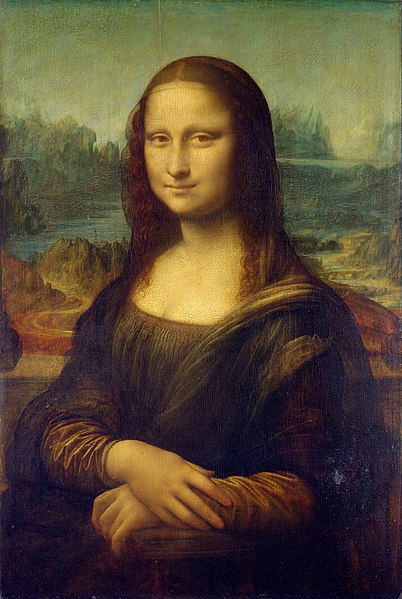
\includegraphics{monalisa}
	\caption[The Mona Lisa]{The Mona Lisa.\\ 
	\url{https://commons.wikimedia.org/wiki/File:Mona_Lisa,_by_Leonardo_da_Vinci,_from_C2RMF_retouched.jpg}}
	\labfig{marginmonalisa}
\end{marginfigure}

In addition, the class is based on \KOMAScript's \Class{scrbook}, 
therefore it inherits all the goodies of that.

\section{What this class does not}
\labsec{doesnot}

As anticipated, further customisation of the book is left to the user. 
Indeed, every book may have sidenotes, margin figures and so on, but 
each book will have its own fonts, toc style, special environments and 
so on. For this reason, in addition to the class, we provide only 
sensible defaults, but if these features are not nedded, they can be 
left out. These special packages are located in the \Path{style} 
directory, which is organised as follows:

\begin{description}
	\item[style.sty] This package contains the specifications of page 
	layout, headers and footers, chapter headings, and the fonts used 
	throughout the document.
	\item[packages.sty] Loads additional packages to decorate the 
	writing with special contents (for instance, the \Package{listing} 
	package is loaded here as it is not required in every book). There 
	are also defined some useful commands to print the same words always 
	in the same way, \eg latin words in italics or \Package{packages} in 
	verbatim.
	\item[references.sty] Some useful commands to manage labeling and 
	referencing, again to ensure that the same elements are referenced 
	always in a consistent way.
	\item[environments.sty] Provides special environments, like boxes. 
	Both simple and complex environments are available; by complex we 
	mean that they are endowed with a counter, floating and can be put 
	in a special table of contents.\sidenote[-2mm][]{See 
	\vrefch{mathematics} for some examples.}
	\item[theorems.sty] The style of mathematical environments. 
	Acutally, there are two such packages: one is for plain theorems, 
	\ie the theorems are printed in plain text; the other uses 
	\Package{mdframed} to draw a box around theorems. You can plug the 
	most appropriate style into its document.
\end{description}

\marginnote[2mm]{The audacious users might feel tempted to edit some of 
these packages. I'd be immensely happy if they sent me examples of what 
they have been able to do!}

In the rest of the book, I shall assume that the reader is not a novice 
in the use of \LaTeX, and refer to the documentation of the packages 
used in this class for things that are already explained there. 
Moreover, I assume that the reader is willing to make minor edits to the 
provided packages for styles, environments and commands, if he or she 
does not like the default settings.


\setpartpreamble{
  \vspace{3cm}
  \begin{center}
  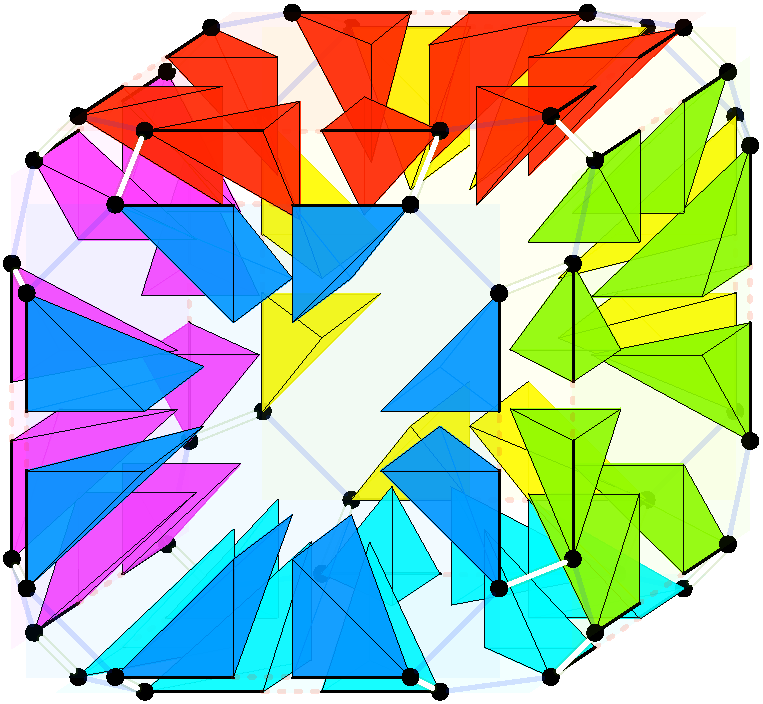
\includegraphics[width=0.8\linewidth]{images/gmaps-3d-simplices}
  \end{center}
}
\newgeometry{top=2.170cm,
			bottom=3.510cm,
			inner=2.1835cm,
			outer=2.1835cm,
			ignoremp}
\part{First Part}
\restoregeometry

\chapter{}

\begin{marginfigure}
	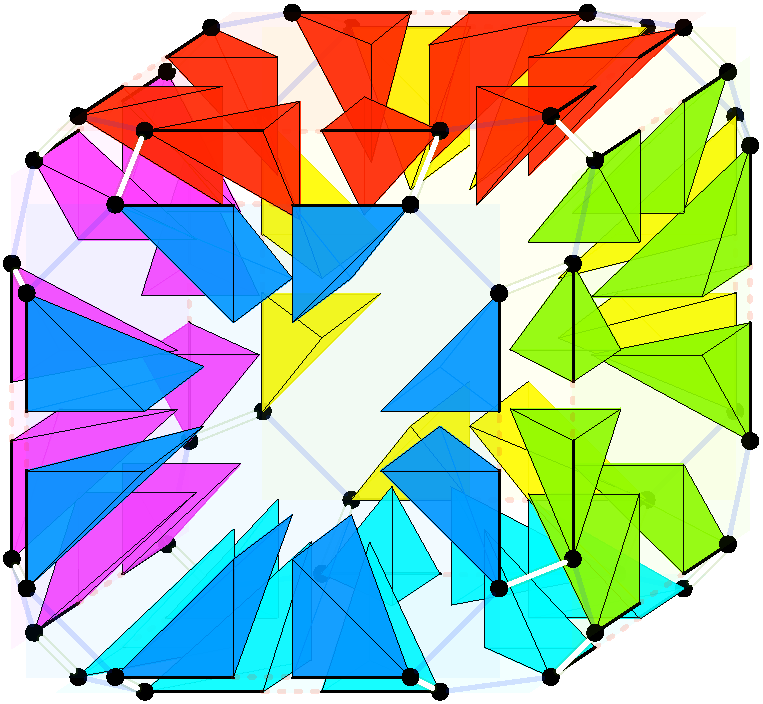
\includegraphics{images/gmaps-3d-simplices}
	\caption{I'm a figure with a footnote}
	\labfig{margin}
\end{marginfigure}

\blindtext

who said footnote? \footnote{ciao \blindtext}


\Blinddocument


\appendix

\blinddocument


\backmatter

% Bibliograhy
\printbibliography[heading=bibintoc,title=Bibliography]

% Glossary
%\printglossaries

% Index
%\printindex

% Back cover
\clearpage
\thispagestyle{empty}
\null%
\clearpage
%\includepdf{pages/cover-back.pdf}

\end{document}
